\documentclass[letterpaper,12pt]{report}
\usepackage[top=1in,right=1in,bottom=1in,left=1.5in,nohead]{geometry}

% PACKAGES
%**********
\usepackage{amsmath}		% AMS Math (http://www.ams.org/tex/amslatex.html)
\usepackage{amssymb}		% AMS Symbols
\usepackage{amsthm}			% AMS Theorems
\usepackage{tocloft}		% Format the Table of Contents
\usepackage{float}			% More float commands
\usepackage{sectsty}		% Format section and chapter headings
\usepackage{graphicx}		% Insert images in eps or pdf format
\usepackage{setspace}		% Line-spacing
\usepackage{algpseudocode}
\usepackage{program}
% Potentially useful packages:
% \usepackage{epsfig}			% For EPS figures
% \usepackage{subfigure}		% For side-by-side figures
% \usepackage{sidecap}		% Put captions on the side of figures
% \usepackage{rotating}		% Rotatiion of figures and tables
% \usepackage{multirow}		% Column and row spanning in tables
% \usepackage{chapterbib}		% Insert bibliograhpy with a simple include command

% Generally, you will not want to edit this file, unless adding a LIST OF ILLUSTRATIONS (or similar)

\renewcommand\contentsname{TABLE OF CONTENTS}
\setlength{\cftbeforetoctitleskip}{0in}
\renewcommand{\cfttoctitlefont}{\large\bfseries}
\renewcommand{\cftaftertoctitle}{}

\renewcommand\listtablename{LIST OF TABLES} % Defines exact text of Title
\setlength{\cftbeforelottitleskip}{1in} % Defines how far down from the margin the title should be placed
\setlength{\cftafterlottitleskip}{0.25in} % Defines how far below the title the first entry will be
\renewcommand{\cftlottitlefont}{\hspace{\fill}\large\bfseries} % This line and the next define that the title should be centered and followed by a line with 'Table' on the left and 'Page' on the right.
\renewcommand{\cftafterlottitle}{\hspace{\fill} \vskip 10mm {\large Table \hspace{\fill} Page}}

\renewcommand\listfigurename{LIST OF FIGURES}
\setlength{\cftbeforeloftitleskip}{1in}
\setlength{\cftafterloftitleskip}{0.25in}
\renewcommand{\cftloftitlefont}{\hspace{\fill}\large\bfseries}
\renewcommand{\cftafterloftitle}{\hspace{\fill} \vskip 10mm {\large Figure \hspace{\fill} Page}}

\renewcommand\cftpartdotsep{\cftdotsep}
\renewcommand\cftchapdotsep{\cftdotsep}
\renewcommand\cftsecdotsep{\cftdotsep}
\renewcommand\cftsubsecdotsep{\cftdotsep}
\renewcommand\cftsubsubsecdotsep{\cftdotsep}
\renewcommand\cftparadotsep{\cftdotsep}
\renewcommand\cftsubparadotsep{\cftdotsep}
\renewcommand\cftfigdotsep{\cftdotsep}
\renewcommand\cfttabdotsep{\cftdotsep}

\setlength{\cftbeforepartskip}{12pt}
\setlength{\cftbeforechapskip}{12pt}
\setlength{\cftbeforesecskip}{12pt}
\setlength{\cftbeforesubsecskip}{12pt}
\setlength{\cftbeforesubsubsecskip}{12pt}
\setlength{\cftbeforeparaskip}{12pt}
\setlength{\cftbeforesubparaskip}{12pt}
	% Lots of special formatting to make the ToC adhere to MU requirements

\begin{document}

\doublespacing % Double line-spacing ( or specify something like \setspacing{1.8} )
\allsectionsfont{\singlespacing} % Only body text needs double spacing, titles can be single spaced

\setcounter{page}{1}    
\pagenumbering{roman}

\thispagestyle{empty}

\vspace*{\fill}
\begin{center}
{\large{\bf EMPIRICAL STUDY OF DEEP NEURAL NETWORK ARCHITECTURES FOR PROTEIN SECONDARY STRUCTURE PREDICTION}} % The title on the Title Page must be in all caps.
\end{center}
%\centerline{\large{\bf PROJECT GOES HERE}}
\vskip 10mm
\centerline{\rule{150mm}{0.2mm}} % You can adjust the length of the horizontal line here.
\vskip 10mm
\centerline{A Thesis presented to} % Choose Thesis or Dissertation
\centerline{the Faculty of the Graduate School}
\centerline{at the University of Missouri}
\vskip 10mm
\centerline{\rule{150mm}{0.2mm}}
\vskip 10mm
\centerline{In Partial Fulfillment}
\centerline{of the Requirements for the Degree}
\centerline{Master of Science} % Change to your degree
\vskip 10mm
\centerline{\rule{150mm}{0.2mm}}
\vskip 10mm
\centerline{by}
\centerline{Ming Du} % Your name on the Title Page must be in all caps.
\centerline{Dr. Yi Shang, Thesis Supervisor} % Edit advisor and choose Thesis or Dissertation
\centerline{May 2017} % The month is required to be capitalized.  Use the month and year of your graduation, not the month and year you defend.
\vspace*{\fill}
	% Input the Title Page (no page number, but counts as roman numeral 'i')
\newpage\null\thispagestyle{empty}\newpage
\newpage
\thispagestyle{empty}

The undersigned, appointed by the Dean of the Graduate School, have 
examined the dissertation entitled: % Choose thesis or dissertation

\vspace{8mm}
\centerline{THE TITLE OF YOUR} % The title on the Title Page must be in all caps.
\centerline{PROJECT GOES HERE}
\vspace{8mm}
\noindent presented by Your Name, % Edit with your name (does not need to be in all caps.)

\noindent a candidate for the degree of Doctor of Philosophy % Change to your degree
and hereby certify that, in their opinion, it is worthy of acceptance.
\vskip 15mm
\centerline{\rule{100mm}{0.2mm}}
\centerline{Dr. Advisor Name} % Edit advisor
\vskip 10mm
\centerline{\rule{100mm}{0.2mm}}
\centerline{Dr. Committee Member} % Edit committee member 1
\vskip 10mm
\centerline{\rule{100mm}{0.2mm}}
\centerline{Dr. Committee Member} % Edit committee member 1
\vskip 10mm
\centerline{\rule{100mm}{0.2mm}}
\centerline{Dr. Committee Member} % Edit committee member 1
\vskip 10mm
\centerline{\rule{100mm}{0.2mm}}
\centerline{Dr. Committee Member} % Edit committee member 1
	% Input the Approval Page (no page number)
\newpage
\pagenumbering{roman}
\setcounter{page}{2}
\addcontentsline{toc}{chapter}{ACKNOWLEDGMENTS} % This is the American english spelling (no E between G and M)

\centerline{\bf \large ACKNOWLEDGMENTS}
\vskip 10mm % Edit everything below with your acknowledging text.
This page is where you would acknowledge all those who helped you with your academic research. This is not necessarily where you would recognize loved ones who supported you during your studies. That would be more appropriately done in an optional Dedication page. I would like to thank Professor Smith � Lorem ipsum dolor sit amet, consectetuer adipiscing elit. Vestibulum eu tellus. Nullam et odio eget sapien porttitor interdum. Donec vel ante. Maecenas in sem a nunc viverra hendrerit. Quisque ut massa quis pede blandit pharetra. \par
Pellentesque sed ligula sit amet ligula scelerisque sagittis. Nulla adipiscing tellus at pede. Cras id nunc vel diam congue dictum. Donec a nulla nec eros ornare consequat. Nullam quis orci. Nam adipiscing, erat in congue pellentesque, dolor eros euismod quam, a egestas mauris magna varius justo. \par
Sed eu sem et lorem blandit volutpat. Duis pulvinar, arcu quis suscipit convallis, ante elit auctor dui, in fermentum diam velit a mauris. In risus odio, consectetuer quis, ullamcorper in, rutrum ut, metus.
	% Input the Acknowledgement Page (roman numeral page number 'ii')
% Only edit this file if you want to include a new list of illustrations, theorems, or other (in which case you will need to add a block to Command_Mods.tex

% Generate a table of contents
\newpage

\singlespacing
\begin{center}
\tableofcontents
\end{center}
\doublespacing

% Generate a list of Tables and a list of Figures:
\newpage
\addcontentsline{toc}{chapter}{LIST OF TABLES}
\listoftables

\newpage
\addcontentsline{toc}{chapter}{LIST OF FIGURES}
\listoffigures
	% Generate and input a Table of Contents and List of Figures/Tables/etc.(roman numeral page number 'iii')

\newpage
\addcontentsline{toc}{chapter}{ABSTRACT}

\centerline{\bf \large ABSTRACT}
\vskip 10mm % Edit everything below with your acknowledging text.
Protein secondary structure prediction is a sub-problem of protein structure prediction. Instead of fully recovering the whole three dimensional structure from amino acid sequence, protein secondary structure prediction only aimed at predicting the local structures such as alpha helices, beta strands and turns for each small segment of a protein. Predicted protein secondary structure can be used for improving fold recognition, ab initial protein prediction, protein motifs prediction and sequence alignment.

Protein secondary structure prediction has been extensively studied with machine learning approaches. And in recent years, multiple deep neural network methods have pushed the state-of-art performance of 8-categories accuracy to around 69\%. Deep neural networks are good at capturing the global information in the whole protein, which are widely believed to be crucial for the prediction. And due to the development of high level neural network libraries, implementing and training neural networks are becoming more and more convenient and efficient.s

This project focuses on empirical performance comparison of various deep neural network architectures and the effects of hyper-parameters for protein secondary structure prediction. Multiple deep neural network architectures representing the state-of-the-art for secondary structure prediction are implemented using TensorFlow, the leading deep learning platform. In addition, a software environment for performing efficient empirical studies are implemented, which includes network input and parameter control, and training, validation,  and test performance monitoring. An extensive amount of experiments have been conducted using popular datasets and benchmarks and generated some useful results. For example,  the experimental results show that recurrent layers are useful in improving prediction accuracy, achieving up to 5\% improvement on 8-categories accuracy.

\newpage
\setcounter{page}{1}
\pagenumbering{arabic}
\addtocontents{toc}{\protect \contentsline {chapter}{CHAPTER}{}}

\chapter{INTRODUCTION}
	\label{CH_Intro}

Accurately and reliably predicting 3D structures, from protein sequences 
is one of the most challenging tasks in computational biology, and has been of great
interest in bioinformatics. An important intermediate step of predicting the whole 3D structure 
is correctly predicting the secondary structure of a protein\cite{yaseen2014context}. In recent years, 
Deep neural networks have been widely apply to the problem of protein secondary structure prediction and continuously pushing the state-of-the-art forward. For example, in\cite{zhou2014deep} a convolutional Generative Stochastic Network achieved 66.4\% Q8(8 categories) on CB513 dataset.  In \cite{Z.Li2016} a convolutional recurrent network which is a combination of convolutional network and recurrent network achieved 69.7\% Q8 accuracy. And in \cite{busia2016protein} they use a multi-scale convolutional network together with many techniques that help accelerating training and prevent over-fitting, such as dropout\cite{srivastava2014dropout}, batch-normalization\cite{ioffe2015batch} and regularization. The best Q8 result they report on CB513 is 70.6\%. 

One advantage of deep learning and deep neural network is the reusability. On one hand, a certain kind of architecture can apply to different problems without much modification. For example, a convolutional recurrent network similar to the one in \cite{Z.Li2016} have also been apply to video activity recognition and Video Description\cite{donahue2015long}. And the convolutional architecture in\cite{busia2016protein} are originally used in image recognition. On the other hand, most complex networks contain reusable modules such as different layers, regularizer and optimizer. So in this case a good way to build a deep neural network is using a reliable deep learning framework such as Torch, TensorFlow Caffe and Theano. TensorFlow\cite{abadi2016tensorflow} is a python deep learning framework create by Google. Using TensorFlow, it easy for researchers to visualize the graph and training process. And the API designs make researchers’ code shareable, standardize how software engineers approach deep learning.

The first goal the this work is to design and build a deep learning system that handles the training, validation, evaluation and save/restore of deep neural networks for protein secondary structure prediction. The second goal is to use the system to compare the performances such as accuracy, running speed and building time of different network architectures.

This thesis will show how to build different deep neural networks using TensorFlow to solve the protein secondary structure prediction problem. And this work will particular focus on how to build a recurrent network and the technique difficulties in doing this. Chapter \ref{CH_02} will introduce the related deep neural network architectures that designed for protein secondary structure prediction, and the mechanism of recurrent neural network. And chapter \ref{CH_03} will describe the models in detail. Chapter \ref{CH_04} will cover the design, implementation and technique difficulties. Chapter \ref{CH_05} will show the result of all the experiments.

\chapter{RELATED WORKS}
	\label{CH_02}


\section{Recurrent networks}
Different from other networks such as feed forward neural network(FFNN) and convolution neural network, recurrent network works well on problems that have sequential input such as speech recognition, language modeling, translation and image captioning. Figure \ref{fig:0} shows how a typical recurrent network looks like. A loop in the network allows it to pass the information from previous steps to the network to make a decision for the current input. In contrast to the fix length context window used in FFNN, RNN stores the activation of previous time step in hidden state and it provide context information within a undefined window size.

\begin{figure}[h] 
	\centering
	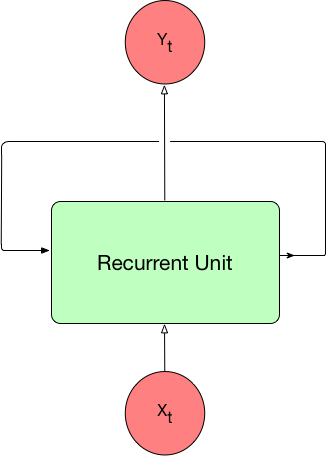
\includegraphics[width=2.0in]{Figures/recurrent1}
	\caption[recurrent network]{Illustration of recurrent network}
	\label{fig:0}
\end{figure}

However, training conventional RNNs using back-propagation technique is difficult due to the vanishing gradient and exploding gradient problems\cite{bengio1994learning}. The gradient shifting problem make
also make it difficult for the network to remember long time dependency that longer than 5-10 time steps between input and output.
\subsection{Long Short term memory}
In order to address the problem above, a special recurrent network architecture Long-Short-Term Memory(LSTM) have been proposed\cite{hochreiter1997long}. LSTM and it's variations have been successfully applied to sequence prediction, translation and sequence labeling tasks. The rest of this chapter will introduce how LSTM and one of its variantion GRU(gated recurrent unit) works.\par

\subsection{Long short term memory}
To make it easier to understand the idea of LSTM, in Figure \ref{fig:1} the loop in the network been unrolled and results in a fix length static version of the same network. The operation in the two RNN version are the same, the difference is the static version only take fix length input and don't have to consider when to stop the iteration thus it runs faster.\par
\begin{figure}[h] 
	\centering
	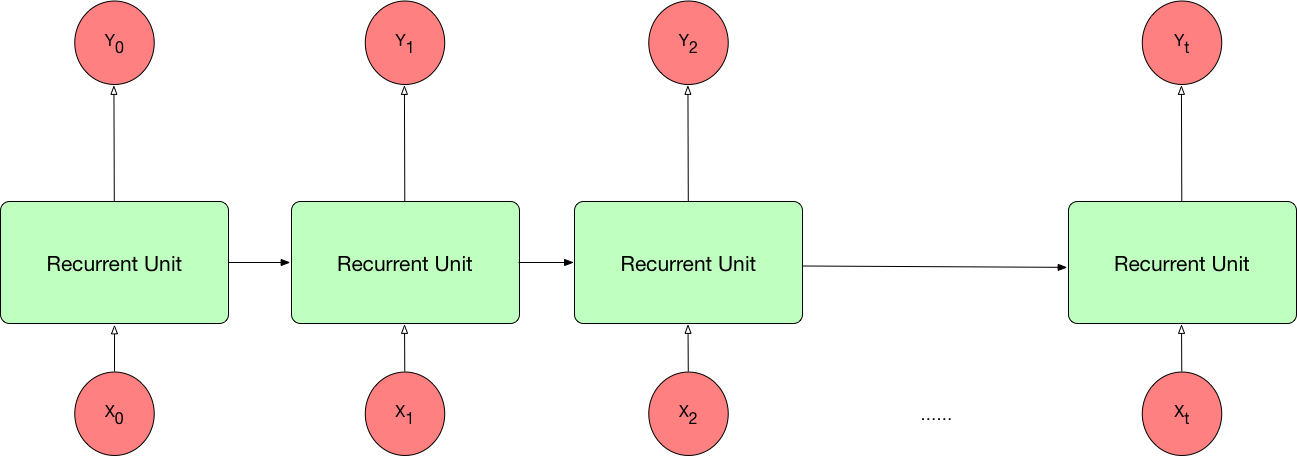
\includegraphics[width=6.0in]{Figures/recurrent2}
	\caption[unrolled recurrent network]{unrolled recurrent network}
	\label{fig:1}
\end{figure}

When we look at the inside of each recurrent unit(Cell), a conventional RNN can be represent as Figure \ref{fig:2}. The cell take the concatenation of input of time t and output of time t-1 as input. Going through a dense layer the cell will output the activation of the dense layer.\par  

LSTM also have the same loop structure of conventional RNN, but it has different structure inside the cell. Instead of having only a single dense layer in the cell, the LSTM cell has four dense layers. One of them is the counter-part in conventional RNN cell, the rest three, however, works as three "gates" controlling the behavior of the cell(Figure \ref{fig:3}).\par 


\begin{figure}[h] 
	\centering
	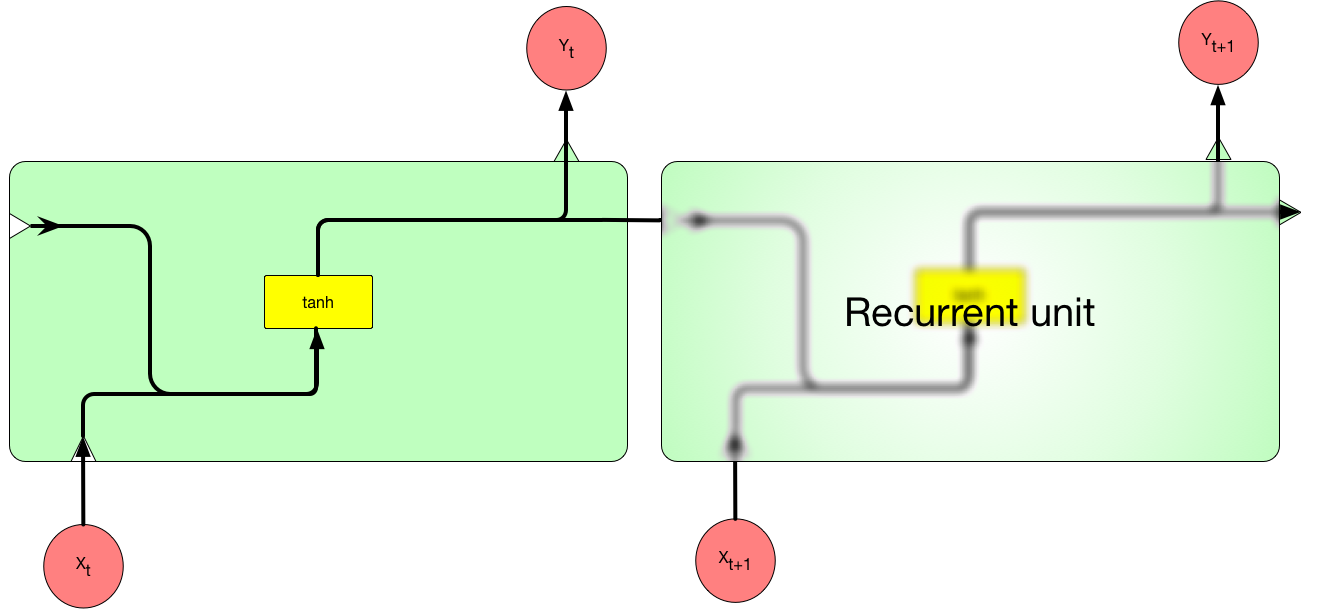
\includegraphics[width=6.0in]{Figures/recurrent3}
	\caption[Detail inside recurrent unit]{Detail inside recurrent unit}
	\label{fig:2}
\end{figure}

\begin{figure}[h] 
	\centering
	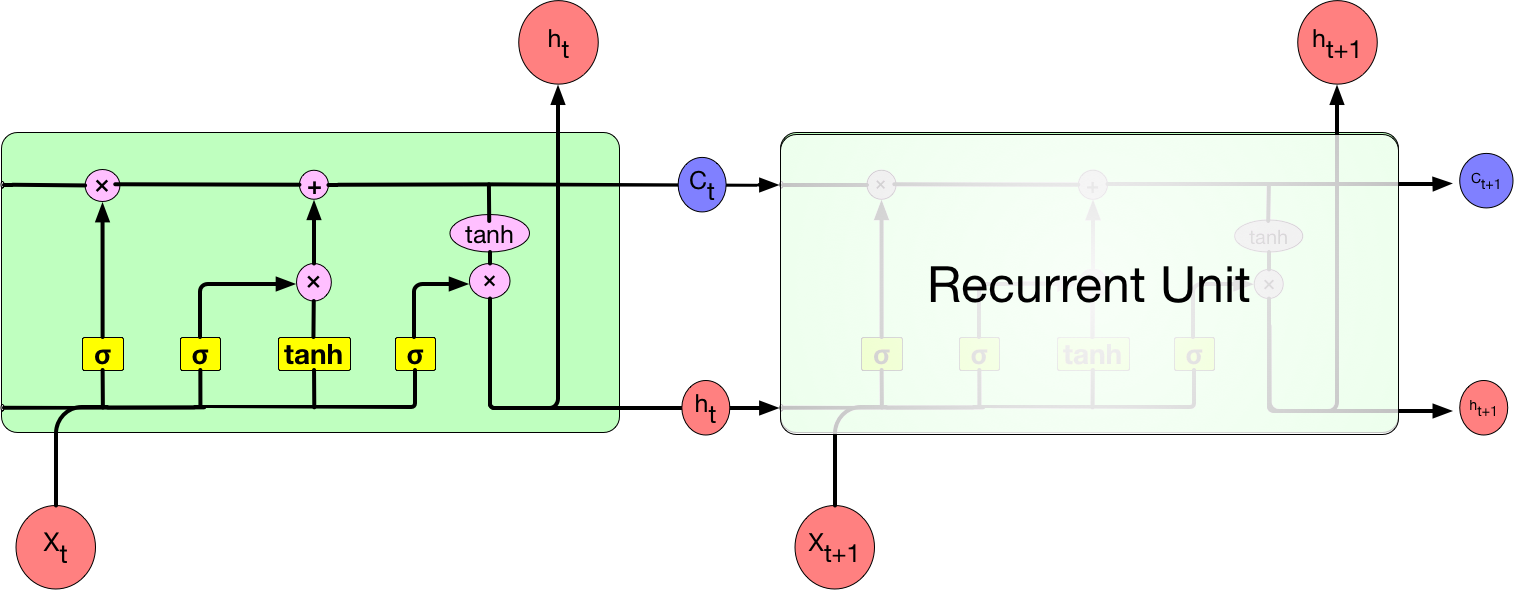
\includegraphics[width=6.0in]{Figures/recurrent4}
	\caption[Detail inside LSTM]{Detail inside LSTM}
	\label{fig:3}
\end{figure}

The first step of calculating the output $h_t$ of each time step is updating the cell state $C_t$. Because the output of each time step is essentially the cell state masked by a weight matrix. In order to update the cell state, the output of the first three dense layer inside the cell needed to be calculated. They are forget gate layer, input gate layer and $tanh$ layer respectively. The activation of these three layers can be calculated by using \ref{eq:0}, \ref{eq:1} and \ref{eq:2}. Then according to  \ref{eq:3} the network will decide how to update the cell state by forgetting some of the old state and remember some of the new input state.\par
After updated the cell state, the network will calculate the output of this time step using \ref{eq:4} and \ref{eq:5}. More specifically speaking, \ref{eq:4} calculate the output gate weights $o_t$ and  \ref{eq:5} apply the weight to the activation of cell state. 
\begin{subequations} 
    \begin{align}
    	f_{ t }&=\sigma (W_{ f }\cdot [h_{t-1} , x_t] +b_f) \label{eq:0}\\	
        i_t &= \sigma(W_i \cdot[h_{t-1}, x_t] + b_i)\label{eq:1}\\
        \tilde {  {C _t } } &= tanh(W_c\cdot [h_{t-1}, x_t]+ b_c) \label{eq:2}
    \end{align}	
\end{subequations}




\begin{equation} \label{eq:3}
    C_t = f_t\ast C_{t-1} +i_t\ast \tilde{C}
\end{equation}

\begin{subequations}
    \begin{align}
        o_t &= \sigma(W_o\cdot [h_{t-1}, x_t] +b_o) \label{eq:4}\\
        h_t &= o_t \ast tanh(C_t) \label{eq:5}
    \end{align}
\end{subequations}

\par


\subsection{Gated recurrent unit}
\par
The gate recurrent unit(GRU)\cite{cho2014learning} is a variance of LSTM. In fact there are many different version of LSTM. The version described in previous chapter is the simplest one. One problem of this LSTM version is that the number of parameters is about 4 times of a conventional recurrent network, because it have four dense layers inside the cell. And it have to keep the cell state which will consume more memory. These problems slow down the speed of the network. The GRU is a special variance of LSTM that only has three dense layer and doesn't have the cell state.\par

\begin{figure}[h] 
	\centering
	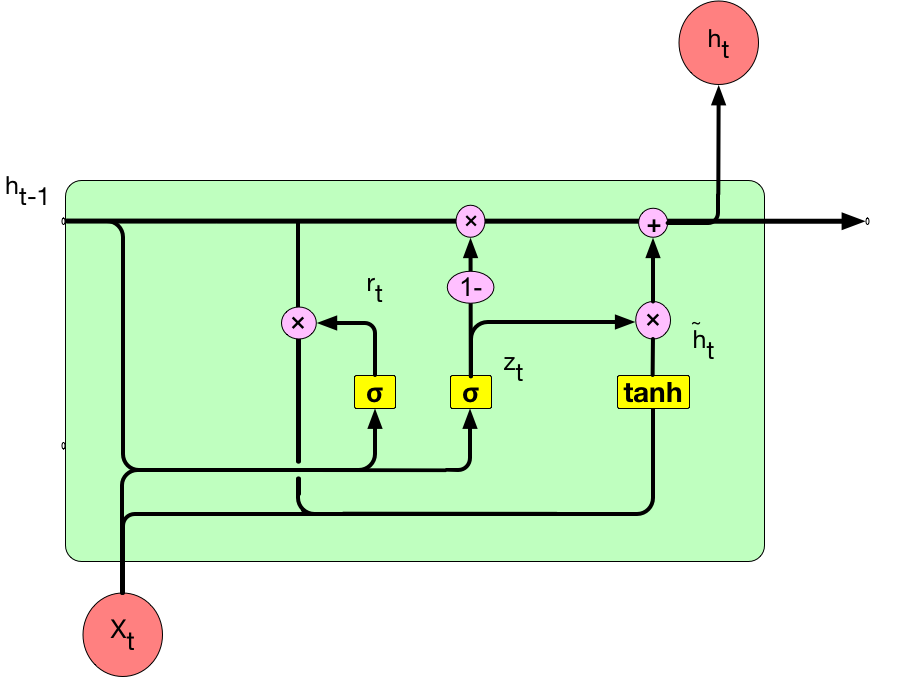
\includegraphics[width=6.0in]{Figures/recurrent5}
	\caption[details in GRU]{details in GRU}
	\label{fig:4}
\end{figure}

As illustrate in Figure \ref{fig:4}, GRU merge the input gate and forget gate in LSTM cell into a single update gate $z_t$. The update gate $z_t$ selects whether the hidden state is to be updated with
a new hidden state $\tilde{h}$. The reset gate $r_t$ decides whether the previous hidden state is ignored. See Eqs. \ref{eq:GRU0}-\ref{eq:GRU1} for the detailed equations of $r, z, h$ and $\tilde{h}$.

\begin{subequations} 
    \begin{align}
    	z_t &= \sigma(W_z\cdot [h_{t-1}, x_t]) \label{eq:GRU0}\\ 
        r_t &= \sigma(W_r\cdot [h_{t-1}, x_t]) \label{eq:GRU1}\\
        \tilde{h} &= tanh(W\cdot [r_t\ast h_{t-1}, x_t]) \label{eq:GRU2}\\
        h_t &= (1 -z_t)\ast h_{t-1} + z_t\ast \tilde{h} \label{eq:GRU3}
    \end{align}	
\end{subequations}

\section{DNNs for protein secondary structure prediction}
Despite some early attempts using neural networks as submodules to predict protein secondary structure such as condition conditional neural fields \cite{wang2011protein}. Several end-to-end trainable deep neural networks have also been proposed to solve the 8-class secondary structure prediction problem. The first one is a convolutional Generative Stochastic Network proposed by Zhou et al.\cite{zhou2014deep}. This method achieved 66.4\% 8-class accuracy on CB513. This model is not very effective since simply using multiple convolutional layers can also achieve 66\% accuracy. The second method, or second kind of architecture is using recurrent network combine with convolutional layers. Søren\cite{sonderby2014protein} and Z.Li et al. \cite{Z.Li2016} both proposed their recurrent neural network and achieved 67.4\% and 69.7\% 8-class accuracy respectively. The major difference of these two method is the first one using 1 layer bidirectional long short term memory(LSTM) cell as recurrent unit, the second one using 3 layers of bidirectional gated recurrent unit(GRU) cell instead. Søren provides the theano source code of the method on github and continues the development, the current best accuracy is 68.9\%. The last architecture is proposed by Busia et al.\cite{busia2016protein}. They stacks multiple convolutional blocks which similar to inception architecture in the network and get 70.6\% accuracy on CB513. Their convolutional model is designed to mimic the behavior of a recurrent sequence to sequence model and is evaluated using beam search. 
% 2. convolutional Generative Stochastic Network achieved 66:4% 
% 3. convolutional recurrent
% 4 google inception net
\chapter{Title of third chapter}
	\label{CH_03}


\section{This is an example section title which will span two lines both here and in the table of contents}
Further illustration of how chapters are presented.


\subsection{Title of subsection}
Here is a subsection.  The following figure will show up in the `List of Figures'.

\begin{figure}[h] % h places the image 'here' (as long as LaTeX thinks it will fit here well), 't' for top of page, 'b' for bottom of page, 'H' for I WANT IT HERE!!! (regardless of whether the latex compiler thinks it will fit.)
	\centering
	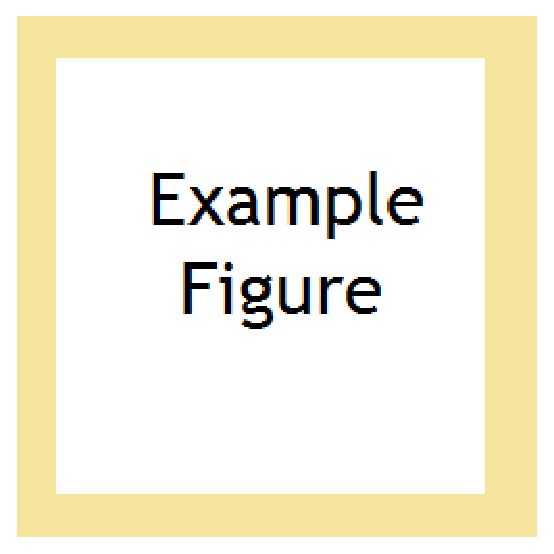
\includegraphics[width=2.0in]{Figures/figure1}
	\caption[Box figure]{A sample image which will show up in the the List of Figures as `Box figure'}
\end{figure}
\begin{table}[t]
	\centering
	\begin{tabular}{|r|l|}
	\hline
	7C0 & hexadecimal \\
	3700 & octal \\ \cline{2-2}
	11111000000 & binary \\
	\hline \hline
	1984 & decimal \\
	\hline
	\end{tabular}
	\caption[Digit representation]{A sample table which will show up in the the List of Tables as `Digit representation table'; it is set to align at the top of a page}
\end{table}

Some paragraph text follows. Some paragraph text follows. Some paragraph text follows. Some paragraph text follows. Some paragraph text follows. Some paragraph text follows. Some paragraph text follows. Some paragraph text follows. Some paragraph text follows. Some paragraph text follows. Some paragraph text follows. Some paragraph text follows. Some paragraph text follows. Some paragraph text follows. Some paragraph text follows. Some paragraph text follows. Some paragraph text follows. Some paragraph text follows. 

\begin{table}[h]
	\centering
	\begin{tabular}{llr}
	\hline
	\multicolumn{2}{c}{Item} \\
	\cline{1-2}
	Animal & Description & Price (\$) \\
	\hline
	Gnat  & per gram & 13.65 \\
	 & each     &  0.01 \\
	Gnu   & stuffed  & 92.50 \\
	Emu   & stuffed  & 33.33 \\
	Armadillo & frozen & 8.99 \\
	\hline
	\end{tabular}
	\caption[Odd foods]{Another table which will show up in the the List of Tables as `Odd foods'; it is set to align ``here" in the text.}
\end{table}




\chapter{DESIGN AND IMPLEMENTATION OF A DNN LEARNING SYSTEM IN TENSORFLOW FOR PROTEIN SECONDARY STRUCTURE PREDICTION}
	\label{CH_04}
Deep learning in these days are not just simply building a model, train it on training set and test it on testing set. On one hand, there is a common trend in recent development of new network architectures. That is modularization, instead of finding a best architecture for a certain task, the most exciting and successful techniques are focusing on finding modules or strategy that can be add to current architectures and improve the performance. For example, dropout and batch normalization are layers that can be add after every activation in order to speed up the learning and prevent overfitting. And residue net and inception \cite{szegedy2015going} construct their structure by stacking modules repeatedly. So a good deep learning program should be able to easily add or remove certain module or function to/from the model. On the other hand, while the network architecture becoming more complex and the dateset getting bigger, the training time are getting longer and often need to run the program on GPU, multi-GPUs or clusters. In order to meet different requirements without changing the program too much, a robust and flexible program are needed. Fortunately, TensorFlow provides excellent building blocks to build such programs and the following sections will introduce the design and TensorFlow implementation of a system that has training, validation, testing, inference, logging, monitoring and save/restore functions.

\section{System design}
\subsection{A brief introduce of TensorFlow mechanism}
The unique way of how TensorFlow works have a huge influence on the system design fashion. So it's important to have some understanding of TensorFow, before introducing the system. \par
There are two major parts in every TensorFlow program, that is graph and session.
\begin{enumerate}
   \item Graph: a computational model contains all the operation you want to perform on the dataset.
   \begin{itemize}
     \item The graph is only a data structure record all the operations that will be executed when data feed into the graph. 
     \item The graph can't run by itself, it need a session to provide the running environment.
     \item Once the graph is finalized, the structure of the graph can not be changed anymore.
   \end{itemize}
   \item Session: encapsulates the environment for a graph to be executed.
   \begin{itemize}
       \item the environment include data input/output, multithread coordinator, save/restore mechanism, logging and monitor. 
       \item Training, validation, and early stopping will handled by session
   \end{itemize}
\end{enumerate}


\subsection{Overall design}
As illustrate in Figure \ref{fig:system}, the system has four module in general:
\begin{enumerate}
   \item Main module: The most important module in the system, contains the network architecture described in Chapter \ref{CH_03}. And inside the main module, there are three sub-modules in order to separate the training validation and inference procedure. This design makes it possible to run the training, validation and inference procedure using different threads and on different devices(CPUs/GPUs). 
   \item Input module: There are several different data input method in TensorFlow(From memory from files etc.). So the input module handles the different input from different source and different formats. This module separate the main module from the data by providing a standard input interface.
   \item Monitor module: This is a utility module that help keep track the training process in real time. This module will run in a separate thread and save requested intermediate results and statistics to log file periodically. And these results can be visualized using TensorBoard in real time.
   \item Save and restore module: It's common for a deep neural network to train for days. And there are also many things can interrupt the training(power down, run out of memory, pause by user etc.). So it's really helpful to have a module to save checkpoint files periodically and  
   restore the training procedure when the user want to continue training.
\end{enumerate}

\begin{figure}[H] 
	\centering
	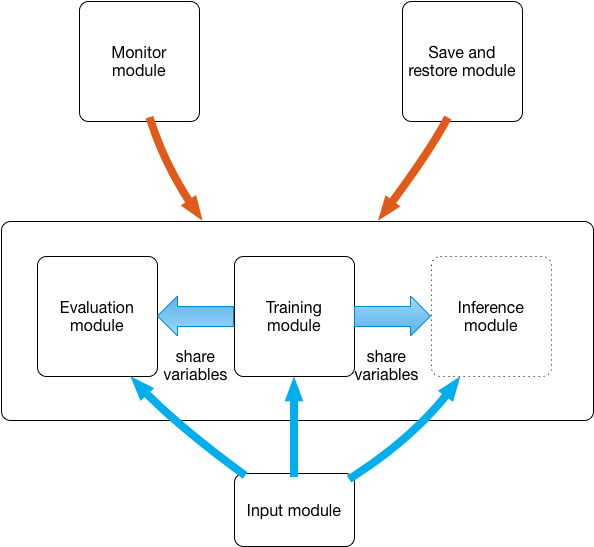
\includegraphics[width=4in]{Figures/system}
	\caption[System overview]{System overview}
	\label{fig:system}
\end{figure}


\subsection{Training, evaluation, inference module design}
Now let's further demonstrate the detail of the main module in Figure \ref{fig:system}. As illustrate in Figure \ref{fig:system_detail} the main module have three different sub-modules, they are training, evaluation and inference. According to different functionality, they have different components. The simplest one is the inference module. This module is only used when user already have a trained model and what to predict the secondary structures for new proteins. The only output is the prediction. The other relative simple one is the Evaluation model, this module is useful when user want to calculate the model performance on certain dataset. So beside prediction, this module also calculate the accuracy and loss. The last module is the training module, which calculate the gradient and update the correspond parameters in the model.\par

The following pseudo code is a pipeline for training a deep neural network. Generally speaking, when training a network, it's better to evaluate the training model in real time. It can save running time by early stopping the training when the model start overfitting or the improvement is really small. Comparing to the method that save a series of candidate best models. This approach also saves disk space, because at each time the system only need to keep two checkpoint files, one file records the current training process, the other records the best model which is the one with the highest validation accuracy.\par


\begin{program}
\mbox{\textbf{ Training pipeline} }
\BEGIN \\ 
\WHILE iteration \lt max\_iteration \DO 
    \CALL |training\.run\_one\_batch|()
    \IF time to validate 
        \CALL |valid_accuracy| = |validation|()
        \IF |valid_accuracy| \gt |best_accuracy|
                  \CALL |save\_model|()
                  best_accuracy = valid_accuracy\FI
    \IF \CALL |should_early|() == |True|
        break
    
\end{program}

The most straightforward way to implement the training pipeline with validation and early stopping is only build one model and switch the input dataset for training or validation. However it's not a good idea in practice. The disadvantages are the following:

\begin{enumerate}
   \item There are different input methods for data in memory and data on hard disk. In FensorFlow you can not switch between this two methods for a single model. Because the input method is part of the Graph and can not be modified once the graph finish building.
   \item If only one model is built for training and validation, the output and statistics of training and validation will be mixed together, since the monitor and output operator is also parts of the TensorFlow Graph, and can not be modified after the building phase. 
   
\end{enumerate}
So with different modules for different purposes in the graph, users can have separate input, output and monitor method for each module. When users want to train a model with validation, they can first build the training module, and then build a Evaluation module with validate dataset. And the two modules are set to share the same model parameters, to make sure the validation module are actually using learned model. When users need test result on test dataset, only a evaluation module will be build with test dataset, and the model will be initialized using saved model on hard disk.
\begin{figure}[H] 
	\centering
	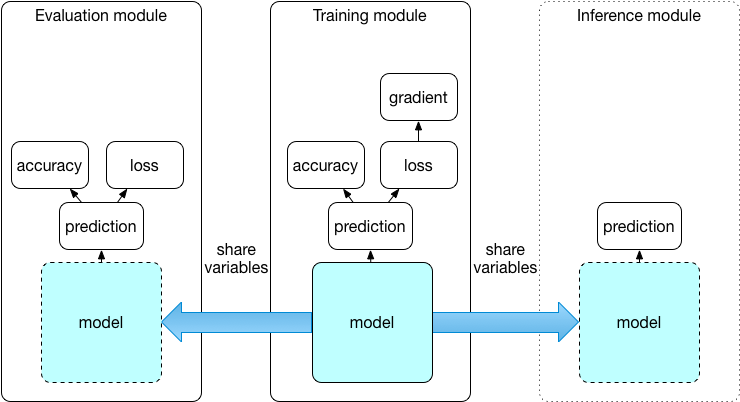
\includegraphics[width=5in]{Figures/system_detail}
	\caption[Detail inside modules]{Detail inside modules}
	\label{fig:system_detail}
\end{figure}

\subsection{Implementation details}
\subsection{Input}
% introduce batch
In the network architecture discussed in Chapter \ref{CH_03}, the input is a single training example. However in practice, the input should always be a batch of multiple examples. In this case, the batch contain 64 protein sequences. And each protein sequence are normalized to 700 hundred length(protein shorter than 700 hundred pad with zeros and protein longer than 700 are cut into segments).  Figure \ref{fig:len_dist} shows the distribution of protein length, the mean value is 208, most of the proteins are shorter than 300. So in each batch, there will be more than half of the data in it are zero paddings. And these zero paddings are actual affect the performance of the network, which will be shown in following sections. So in order to deal with zero paddings, besides the original input data, the length of each protein will also add to each batch. So each batch will have a shape of [64, 700, 42 + 1].

\begin{figure}[H] 
	\centering
	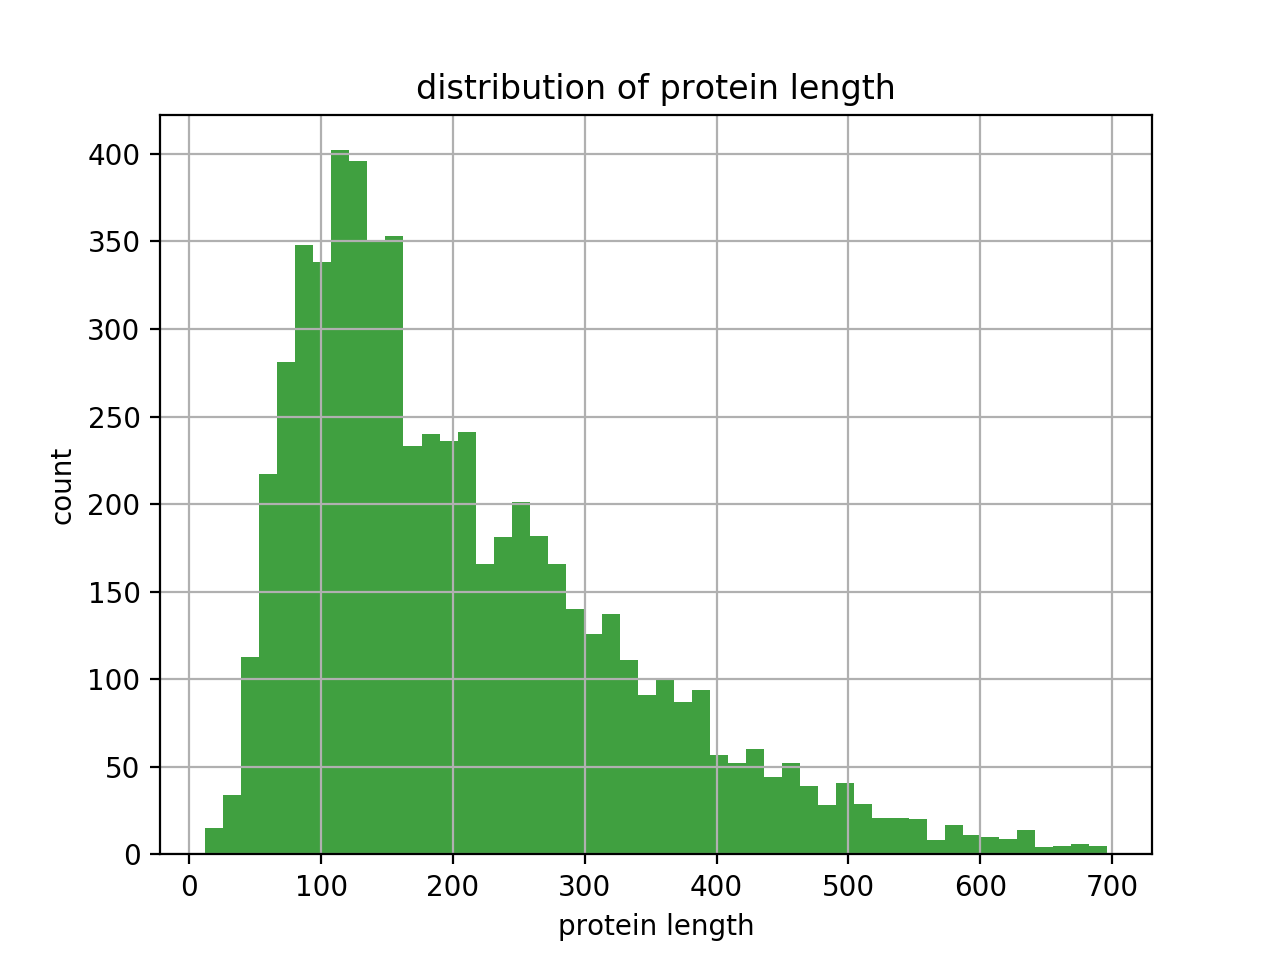
\includegraphics[width=5in]{Figures/length_distribution}
	\caption[Distribution of protein length]{Distribution of protein length}
	\label{fig:len_dist}
\end{figure}

There are two major data input method in general. Input data from memory and input data from disk. The most popular way you will found in TensorFlow tutorials or examples are input data from memory. That is read all the data into memory and prepare each batch by your self. This method is easy to use, and user have more control of the input process. However when you can not put all the data into memory, this method is inadequate. TensorFlow also provides a build-in method for reading data from file. Users can convert all data into TensorFlows default binary format, or provide reader functions. Then TensorFlow will help you handle the data input process, as long as user provides the list of input file names. As illustrate in Figure \ref{fig:input}, a file name queue and a data queue are built as input buffer. For each step the model will read a batch from the data queue. 

In this project, training module is using the file input pipeline. However evaluation module is using the light weight memory input method, since testing and validation data are usually have small size and only need to scan through the data only once for evaluation. 

\begin{figure}[H] 
	\centering
	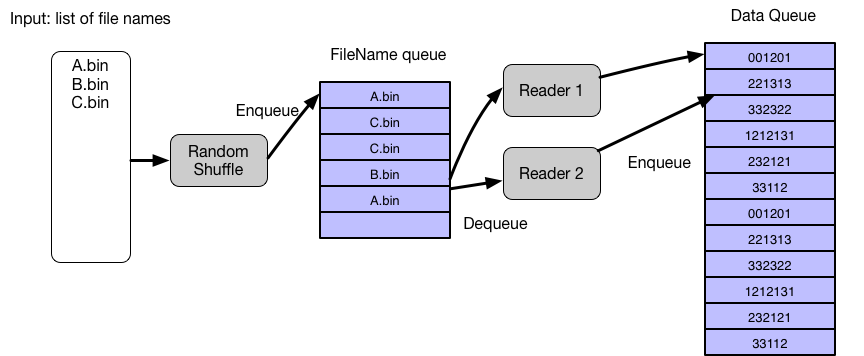
\includegraphics[width=5in]{Figures/input}
	\caption[Input Queues]{Input Queues}
	\label{fig:input}
\end{figure}


\subsection{Multi-scale convolution}

\subsection{Recurrent layer}
When implementing the recurrent layer, there are two things should be considered. 
\begin{enumerate}
   \item Use dynamic RNN or a static RNN.
   \item When shoul RNN stop calculating for each batch.
\end{enumerate}
In TensorFlow and most other deep learning libraries, there are two common RNN versions: static RNN and dynamic RNN. Dynamic RNN is pretty much what RNN should be like, it use a loop structure to process variable length of sequences. The static one, however, unrolls the loop and have a fixed number of computational nodes to process fixed length sequences, just as what Figure \ref{fig:1} shows. \par
The benefits of using static RNN is it runs faster than a dynamic RNN, since it doesn't have to test the terminate condition for each time step. The actual speed comparison is listed in Table \ref{tb:rnn0}. What's more it is the only RNN implementation in early version of TnesorFlow. The problem of static RNN is that it makes the model too big. A big model have a lot of disadvantages. It use too much memory, both GPU and CPU memory, it consume more disk space to store the best model, and it takes more time to build the model. In this project the 700  sequence length 3 layers with 64 units model will some how use 20G memory and over 4G GPU memory. Comparing to the 4MB model file of dynamic RNN, It took 275MB to store the static model described above, which will slow down the training process every time it same the current best model. And the build time is longer than 10 minutes comparing to the several seconds of dynamic RNN's build time.\par

The reason using a dynamic RNN is that it can adapt to different input and network architectures. Such as sequence to sequence model, which needs the encoder and decoder to be able to handle variable length sequences. When dealing with real life data, a model that accepts variable length input are general easier to use. The dynamic RNN is light weight, flexible and can achieve comparable speed of a static RNN(In table \ref{tb:rnn0} the dynamic rnn is about 8\% slower than the static one).\par
\begin{table}[h] \label{tb:rnn0}
	\centering
	\begin{tabular}{lllrrr}
	\hline
	\multicolumn{3}{c}{Model} &
	\multicolumn{3}{c}{Performance}\\
	\cline{1-3}
	Multi conv & RNN  & Output layers &  Build time (s) &   \begin{tabular}{@{}c@{}}speed \\(batch/s)\end{tabular} & test accuracy(\%)\\
	\hline
	32 channels &- &conv 11  &0.69 &5.28 &65.3\\
	64 channels &- &conv 11  &0.72 &3.44 &65.7\\
	64 channels & \begin{tabular}{@{}c@{}}1 layer \\ static 32\end{tabular} &conv 11 &166.61 &0.77 &-\\
	64 channels & \begin{tabular}{@{}c@{}}1 layer \\ dynamic 32\end{tabular} &conv 11 &1.43 &0.71 &68.7\\
	64 channels & \begin{tabular}{@{}c@{}}1 layer \\ dynamic 2\end{tabular} &conv 11 &1.43 & 0.76 &67.8\\
	64 channels & \begin{tabular}{@{}c@{}}1 layer \\ dynamic 10\end{tabular} &conv 11 &1.47 & 0.758 & 68.3\\
	64 channels & \begin{tabular}{@{}c@{}}1 layer \\ dynamic 128\end{tabular} &conv 11 &1.41 &0.54 & 69.2\\
	64 channels & \begin{tabular}{@{}c@{}}2 layer \\ dynamic 128\end{tabular} &conv 11 &1.94 &0.27 &69.5\\

	\hline
	\end{tabular}
	\caption[Comparison of Static and Dynamic RNN]{Comparison of Static and Dynamic RNN}
\end{table}

Another important detail about RNN is when to stop the iteration. Continuing the iteration after reach the end of the sequence is inefficient, and may cause error when doing back propagation, since the network will try to learn the zero paddings that are irrelevant to the protein sequence. The problem is that proteins in each batch will have different length, so in order to stop the iteration correctly, it is required to provide the length information for every protein in the batch.\par

In summary, RNN layers in this project are dynamic bidirectional RNN, and provided with sequence length information for each sequence in the batch. The unit number of the RNN cell is 128.

\subsection{Output layers}
There are two 1D convolution layer are build after RNN layers. The first one use kernel shape [1] and output channel size is half of the input channel size. The second layer use kernel shape [7] and the output channel is 14.\par
\subsection{loss function}
Different from convolution networks, RNN need several additional steps to calculate the correct average loss value for each batch. Because RNN always deals with variable length data, such as English sentences and ,in this project, proteins. As illustrate in Figure \ref{fig:loss} the output of the network would be a 3D array with shape [batch\_size, sequence\_length, feature\_length]. As you may notice in the figure, there are blanks at the end of each sequence, those are zero paddings. Due to the variable length input data, the blanks are always exist. And consider the distribution in Figure \ref{fig:len_dist}, over half of the data in a batch are zeros. The correct loss function for individual sequence is Equation \ref{eq:loss}. However in practice, due to the parallel feature of TensorFlow, it is required to calculate the loss for all the sequence in a batch at the same time. The result of the batch loss operation is a 2D array with shape [batch, sequence]. Each element in this array is the loss of a single amino acid. After calculating the loss array, a mask array is constructed using the length vector on the left of Figure \ref{fig:loss}. Apply the mask array to the loss matrix will set the loss of the blanks to zero. Finally the average loss per amino acid will be $sum(LOSS\_ARRAY)/sum(length\_vector)$.\par

\begin{figure}[H] 
	\centering
	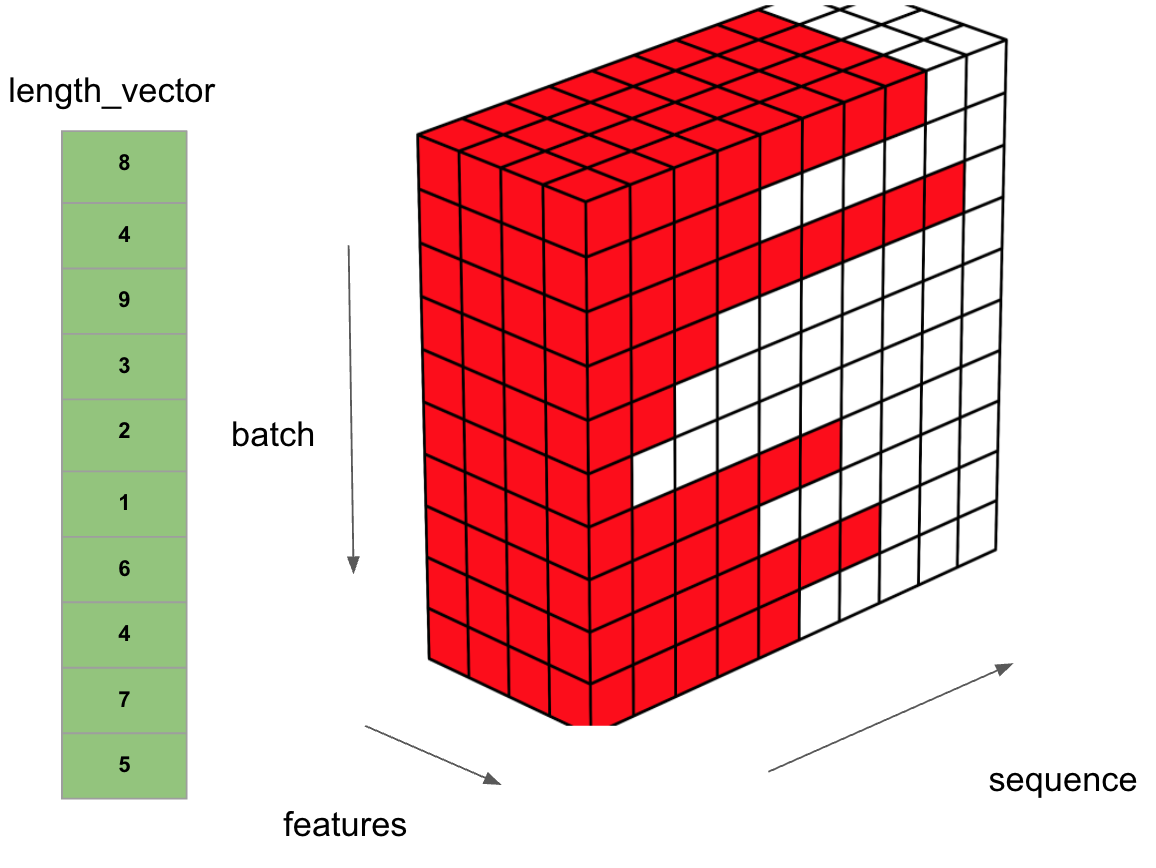
\includegraphics[width=5in]{Figures/loss}
	\caption[Variable length batch Input]{Variable length batch Input}
	\label{fig:loss}
\end{figure}

\subsection{Accuracy operator}
The evaluation of the project is 8 classes accuracy(Q8). The algorithm of calculating Q8 accuracy from predictions and labels is the following.\newline

\begin{algorithm}[H] 
 \KwData{\\Prediction [batch\_size, seq\_len, feature\_len]\\label [batch\_size, seq\_len, feature\_len]\\length\_vector [batch\_size, 1]}
 \KwResult{Q\_8: real number}
    conf\_mat = Confusion\_Matrix(label, prediction)\;
    true\_positive = sum(diag(conf\_mat))\;
    Q\_8 = true\_positive/sum(length\_vector)\;
 \caption{Q8 accuracy }
\end{algorithm}
\vspace{0.5cm}
The implementation of this part is some how tricky. Because when users train the network, they want to monitor the training and validation accuracy in TensorBoard and TensorBoard only monitors the operator inside the Graph. So whatever calculate the accuracy should be an operator inside the TensorFlow Graph. And it should not be a python function outside the Graph. So the correct implementation here is constructing a accuracy operator using basic TensorFlow operators, and add it to the model. Then the calculation will perform inside the Graph and inside GPU. For more details see the code in Appendix.\par

\subsection{Training Monitor}
The actual monitor of the system has two separate parts. The first part is the summary operators inside the TensorFlow Graph which save the value of desired tensors in log files periodically. The tensors(variables) that are monitored in this projects are the following:

\begin{multicols}{2}
  \begin{enumerate}
  \item training module
  \begin{itemize}
    \item training loss
    \item training accuracy
  \end{itemize} 
  
  \item validation module
  \begin{itemize}
    \item validation loss
    \item validation accuracy
  \end{itemize}
  
  \item Input module
  \begin{itemize}
      \item input queue occupancy
      \item running speed (batch/sec)
  \end{itemize}
  \item Distributions and histogram
  \begin{itemize}
      \item output of Multi CNN
      \item output of RNN layers
  \end{itemize}
  \end{enumerate}
\end{multicols}
The second part is a visualization tool called TensorBoard. It a command line tool come with the TensorFlow library. What it dose is reading the log file from the path you provide, and start to host a web page(Figure \ref{fig:monitor}) which have all the graphs on it. The web page will refresh periodically, so users can use the web page as a real time monitor of the training process. The advantage of using TensorBoard is the flexibility. Users can choose when they want the visualization, one can easily turn off the monitor without interrupting the training. And users can also choose where they wan to put the visualization, a model may be trained on a server, and the use can monitor the training by visiting the web page on other computers. 
\begin{figure}[H] 
	\centering
	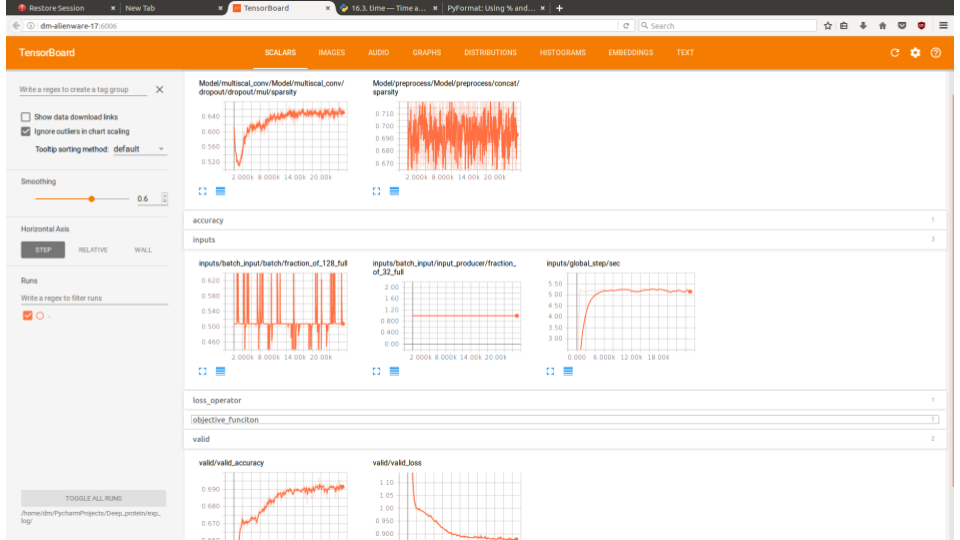
\includegraphics[width=5in]{Figures/monitor}
	\caption[Tensorboard visualization]{Tensorboard visualization}
	\label{fig:monitor}
\end{figure}

\subsection{Save and Restore}
The system saves checkpoint files periodically, since the training process usually take hours to complete, it's important to only keep the newest N checkpoints files. In this project, when training the system will check if there are more than 5 checkpoint files, if true then delete the oldest one. When the system restore training, it will search for the newest checkpoint file and start the training from there. Another file need to save is the best model file, it similar to a checkpoint file, but it only save the trainable parameters instead of all the variables inside the model that are needed to restore training.
\chapter{experiments and results}
	\label{CH_05}
\chapter{SUMMARY}
	\label{CH_summary}
The major achievements of this work is the following:
\begin{enumerate}
    \item Design and implement a DNN learning system in TensorFlow for PROTEIN SECONDARY STRUCTURE PREDICTION.
    \item Provide detailed information on how to use RNN correctly.
    \item Test and explore the trade off between speed and accuracy of the RNN.
    \item Achieve 69.5\% accuracy on CB513, which is comparable to current state-of-the-art.
\end{enumerate}
This work, following the basic network architecture in \cite{Z.Li2016}, use bidirectional GRU RNN after multiscale convolutional layers. Instead of using the exact architecture in their work which has 3 RNN layer and 600 hidden units in each layer. Only 2 128-hidden-unit RNN layers have been used, due to the insufficient GPU memory. However, by using less layers and less hidden units and add batch normalization to the network. The network managed to achieve comparable performance on dataset CB513. The best Q8 accuracy is 69.5\% which is 0.2\% lower than theirs. However, because of the smaller model, it need less time to train the model. This thesis also shown how to design and build a system to train a recurrent network with variable length inputs.\par

The recurrent structure can capture the global context information in the protein sequence and boost the performance of protein secondary structure prediction. However it can not fully capture the context information, simply stack the RNN layer can not out perform a single RNN layer with convolutional layers after it. A possible reason is the current off-the-shelf RNN structures can not deal with extremely long dependencies such as the average 230 length proteins. But there are huge potential in RNN networks. More powerful but complex RNN architectures such as RNN with attention mechanism\cite{luong2015effective} and RNN with batch normalization\cite{cooijmans2016recurrent} may be able to solve this problem. 

\newpage
\addcontentsline{toc}{chapter}{APPENDIX}
\appendix

\chapter{Title of first appendix}
	\label{AP_01}

\section{Section title}
Here is some additional information which would have detracted from the point being made in the main article.
\subsection{Subsection title}
This section even has subtitles
\newpage
\addcontentsline{toc}{chapter}{BIBLIOGRAPHY}

\bibliographystyle{unsrt}
\bibliography{bibtex_entries}

\newpage
\addcontentsline{toc}{chapter}{VITA}

\centerline{\bf \large VITA}
\vskip 10mm % Edit everything below with your acknowledging text.
This is a summary of your {\it professional} life, and should be written appropriately.  This can be written in the following order:  where your where born, what undergraduate university you graduated from, if you received a masters, and which institution you graduated from with your PhD (University of Missouri).  You can describe when you began research with your current advisor. \par
In another paragraph, you could say if/when you were married, what the name of your kids are, and what your plans are for after graduation if you choose.  Take a look at other vita's from other dissertations for examples.


\end{document}